\chapter{Introduction}
Tuatschin is the Sursilvan dialect that differs the most from the standard variety. These differences, however, do not concern the most salient typological features of Sursilvan as e.g. the predicative \textit{-s} of masculine singular adjectives and participles (see § 3.3.1 and 4.1.2.1 below), nouns and adjectives with stem alterations as \textit{iart} (sg) vs \textit{òrts} (pl) `garden(s)' and \textit{matgiart} (sg) vs \textit{macòrts} (pl) `ugly', or the conservation of the Latin diphthong \textsc{au} as in \textit{aur} `gold'.

Some differences between Tuatschin and Standard Sursilvan concern palatalization phenomena, the treatment of monophthongs and diphthongs, some pronominal and verbal forms, the form of the negator, or the form of the dative marker. \tabref{difstand} lists some of these differences.


\begin{table}
	\caption{Differences between Tuatschin and Standard Sursilvan}
	\label{difstand}
	\begin{tabular}{lllll}
		\lsptoprule
		& Tuatschin &  Sursilvan & English\\
		\midrule
	palatalization of ˈ\textsc{ka}  & \textit{marˈʨaw} & \textit{marˈkaw} & `city'\\
	& \textit{ˈʨɛzɐ} & \textit{ˈkazɐ} & `house'\\
	Surs. \textit{ɔ} before \textit{n} & \textit{aˈvawn} & \textit{aˈvɔn} & before\\
	\textsc{1sg} pronoun & \textit{ju} & \textit{jɛw} & `I'\\
	negator	& \textit{ˈbeʨɐ} &  \textit{ˈbukɐ} & `not'\\
	dative marker & \textit{da} &  \textit{a}\\
				\lspbottomrule
	\end{tabular}
\end{table}


\figref{fig:surs} shows the whole territory where Sursilvan is spoken. The Tujetsch valley is located to the west of the territory. The white parts in \figref{fig:surs} correspond to regions where traditionally Swiss German (Walser) dialects are spoken. The orange and yellow parts correspond to regions where Sutsilvan is spoken and belong thus not to the Surselva.

\begin{figure}
	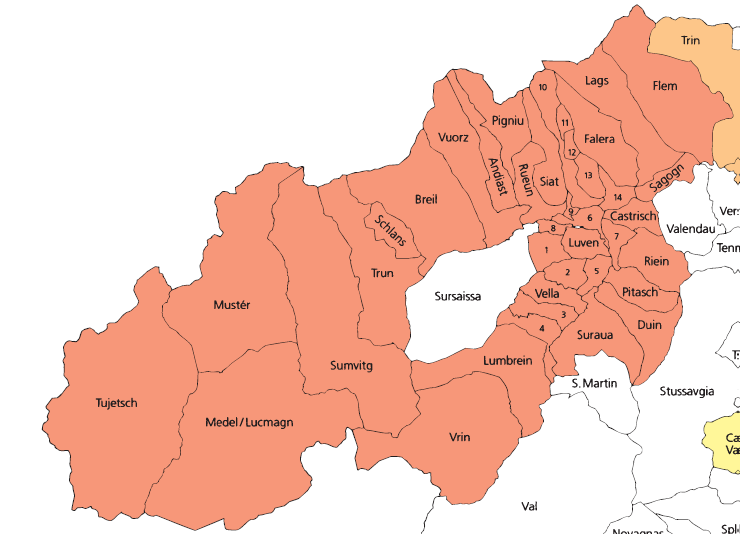
\includegraphics[height=.5\textheight]{figures/Surselva.png}
	\caption{Surselva}
	\label{fig:surs}
\end{figure}


\section{Previous works}
The most important linguistic study about Tuatschin is  \citet{Caduff1952}, \textit{Essai sur la phonétique du parler rhétoroman de la Vallée de Tavetsch}, which is about diachronic phonetics from Latin to Tuatschin. Some indication about Tuatschin can also be found in \citet{VicHendry2010}, \textit{Tujetsch, ses vallers e lur tschontscha}, and \citet{Maurer2017} analyses the marking of the indirect object from a diachronic perspective. 

There are some works containing Tuatschin texts and sentences; these will be mentioned in § 1.2 below.

\section{Corpus}
The corpus consists of oral and written sources. The oral corpus has been collected by myself during different field trips between 2016 and 2020 with 7 female and 10 male native speakers of Tuatschin; it consist of approximately 60 minutes of recorded stories told by male and female consultants between 30 and 82 years of age at recording time, as well as of elicited forms and sentences.

Since I have a working knowledge of standard Sursilvan, all the interviews were conducted in Romansh.

The most important collection of Tuatschin texts is \citet{Büchli1966}, \textit{Mythologische Landeskunde von Graubünden. 2. Teil: Das Gebiet des Rheins vom Badus bis zum Calanda}, which contains about 60, mostly short, traditional stories from the Tujetsch valley (with indication of the village the story tellers were from) which were transcribed by the author himself. Büchli's consultants were born between 1858 and 1922.

The oldest texts I have access to is \textit{Il ratun tschiec} `The blind rat', which was published in 1889, and a transcribed text from the Schorta collection  (\citet{Schorta1926}), republished in \citet{Valär2013a} and \citet{Valär2013b}. Some sentences and dialogues can be found in the \textit{Dicziunari rumantsch grischun}, in \citet{Gartner1910}, \citet{Gadola1935}, Francestg \citet{Berther1998}, and in Baseli \citet{Berther2007}. 

The examples taken from the written sources will all be adapted to the spelling system used in this book, with one exception: those written in IPA.
  
The names of the consultants who participated in the project are made anonymous; their utterances will be labelled with a reference to their sex (m, f) and the place where they grew up. The native speakers of Tuatschin are listed in \tabref{tab:consultantsI} to \tabref{tab:consultantsV}.

\begin{table}
	\caption{List of consultants I}
	\label{tab:consultantsI}
	\begin{tabular}{lllll}
		\lsptoprule
		& f1 & f2 & f3 & f4\\
		\midrule
		born & 1923 & 1937 & 1942 & 1947\\
		grew up in & Cavòrgja & Sèlva & Sadrún & Ruèras \\
		L1 mother & Tuatschín & Tuatschín & Tuatschín & Tuatschín \\
		L1 father & Tuatschín & Tuatschín & Tuatschín & Tuatschín \\
		\lspbottomrule
	\end{tabular}
\end{table}

\begin{table}
	\caption{List of consultants II}
	\label{tab:consultantsII}
	\begin{tabular}{llll}
		\lsptoprule
		& f5 & f6 & f7 \\
		\midrule
		born &  1961 & 1971 & 1972 \\
		grew up in &  Surajn &  Camischùlas &  Ruèras  \\
		L1 mother & Tuatschín & Tuatschín & Tuatschín\\
		L1 father & Sursilvan & Tuatschín & Tuatschín\\
		\lspbottomrule
	\end{tabular}
\end{table}

\begin{table}
	\caption{List of consultants III}
	\label{tab:consultantsIII}
	\begin{tabular}{lllll}
		\lsptoprule
		& m1 & m2 & m3 & m4\\
		\midrule
		born & 1935 & 1934 & 1943 & 1949 \\
		grew up in & Ruèras & Zarcúns & Ruèras & Sadrún\\
		L1 mother & Tuatschín & Tuatschín & Tuatschín & Tuatschín\\
		L1 father & Tuatschín & Tuatschín & Tuatschín & Tuatschín\\
		\lspbottomrule
	\end{tabular}
\end{table}

\begin{table}
	\caption{List of consultants IV}
	\label{tab:consultantsIV}
	\begin{tabular}{lllll}
		\lsptoprule
		& m5 & m6 & m7 & m8\\
		\midrule
		born & 1952 & 1951 & 1953 & 1977\\
		grew up in & Sadrún & Sadrún & Cavòrgja & Sadrún\\
		L1 mother & Tuatschín & Tuatschín & Tuatschín & Tuatschín \\
		L1 father & Tuatschín & Tuatschín  & Tuatschín & Tuatschín\\
		\lspbottomrule
	\end{tabular}
\end{table}

\begin{table}
	\caption{List of consultants V}
	\label{tab:consultantsV}
	\begin{tabular}{lllll}
		\lsptoprule
		& m9 & m10\\
		\midrule
		born   & 1986 & 1943\\
		grew up in   &  Sadrún & Ruèras \\
		L1 mother & Tuatschín & Tuatschín\\
		L1 father  & Tuatschín & Tuatschín\\
		\end{tabular}
\end{table}

All consultants speak Tuatschin, standard Sursilvan, standard and Swiss German, and they are used to write in standard Sursilvan and in standard German. The young generation also uses Tuatschin in SMS and other social media.

Some decades ago, the people from Tujetsch would not use their own dialect with people from outside the Tujetsch valley, and still today some people are not used to speak Tuatschin with somebody who speaks Standard Sursilvan or another Sursilvan dialect. One of my consultants puts it this way:

\ea
\label{}
\langinfo{Tuatschín}{Zarcúns}{m2}\\
\gll I drùva schòn in téc tg' ins, da saprèndar ansjaman da raṣdá da Tujétsch cun autars.\\
\textsc{expl} need.\textsc{prs.3sg} indeed \textsc{indef.art.m.sg} little \textsc{comp} \textsc{gnr} \textsc{comp} \textsc{refl}.take.\textsc{inf} together \textsc{compo} talk.\textsc{inf} of \textsc{pln} with other.\textsc{m.pl}\\
\glt `It needs indeed a little that one, to concentrate in order to speak Tuatschin with others.'
\z

This explains in part why my consultants sometimes use Sursilvan forms when speaking with me.

\section{Dialectal differences}
There are two main Tuatschin dialects: the dialect of the upper part of the Tujetsch valley, which comprises the villages of Selva and Tschamut\footnote{According to DRG 7: 636, the inhabitants of Selva and Tschamut are called \textit{quèls dadajns gl uaut} `those above the forest'; the forest dividing the two parts of the valley is called \textit{Uaut Tschapina}.}, and the dialect of the lower part of the valley, from Dieni to Bugnei. These two dialectal areas are divided by a forest, the forest of Sontga Brida (see \citet[3]{Caduff1952}). The differences are mostly lexical, whereby the divergent forms of the upper dialect correspond in general to Standard Sursilvan. Some examples are presented in \tabref{difdial} (see \citet[97]{VicHendry2010}).

\begin{table}
	\caption{Differences between the upper and the lower dialect}
	\label{difdial}
	\begin{tabular}{lllll}
		\lsptoprule
		Lower valley &  Upper valley and Sursilvan & English\\
		\midrule
		\textit{anavaun} & \textit{anavon} & `forward' \\
		\textit{cuntjants} & \textit{cuntents} & `happy' \\
		\textit{sjantar} & \textit{suenter} & `after'\\
		\textit{tgaglja} & \textit{caglia} & `bushes'\\
		\textit{ufaun} & \textit{affon} & `child' \\
		\lspbottomrule
	\end{tabular}
\end{table}

Nowadays there are only very few speakers of the upper dialect left; an example of the variety of Selva is presented in § 9.6 below.


\section{Glosses}
The glosses used in this grammar are those of the Leipzig Glossing Rules\footnote{https://www.eva.mpg.de/lingua/resources/glossing-rules.php}, whereby some glosses which are not listed in these rules have been added.

In order to save space, gender and number are only indicated on the first element of the noun phrase, excepted in cases where two or more elements of a noun phrase differ in gender and/or number. Indicative mood is not indicated, in contrast to subjunctive, conditional, and imperative mood.

\section{Place names}
In the Romansh examples and texts, I will use the spelling system of this book for the place names. In the English text, I will use the official Sursilvan spelling.

I will not use the German equivalents of the Romansh place names, except if they are used by the consultants themselves.

The place names which occur in this book are indicated in \tabref{spellpln}. The German equivalents are only given for those place names that are located in German speaking areas.

\begin{table}
	\caption{Spelling of place names}
	\label{spellpln}
	\begin{tabular}{lllll}
\lsptoprule
current spelling &  Standard Sursilvan & German\\
\midrule
\textit{Bugnaj} & \textit{Bugnei}\\
\textit{Camischùlas} & \textit{Camischolas}\\
\textit{Caṣchinùta} & \textit{Caschinutta} & \textit{Göschenen}\\
\textit{Cavòrgja} & \textit{Cavorgia}\\
\textit{Cuéra} & \textit{Cuera} & \textit{Chur}\\
\textit{Diani} & \textit{Dieni}\\
\textit{Gjònda} & \textit{Gonda}\\
\textit{Gljòn} & \textit{Glion}\\
\textit{Nòssadunaun} & \textit{Nossadunnaun} & \textit{Einsiedeln}\\
\textit{Ruèras} & \textit{Rueras}\\
\textit{Sadrún} & \textit{Sedrun}\\
\textit{Sèlva} & \textit{Selva}\\
\textit{Surajn} & \textit{Surrein}\\
\textit{Trùn} & \textit{Trun}\\
\textit{Tschamùt} & \textit{Tschamutt}\\
\textit{Turitg} & \textit{Turitg} & \textit{Zürich}\\
\textit{Ursèra} & \textit{Ursera} & \textit{Andermatt}\\
\textit{Zarcúns} & \textit{Zarcuns}\\
\lspbottomrule
\end{tabular}
\end{table}

Gjònda: Geröllhalde, unproduktives Gelände
